\documentclass[10pt,draftclsnofoot,onecolumn,compsoc]{IEEEtran}
\usepackage[letterpaper, portrait, margin=0.75in]{geometry}
%\usepackage[myheadings]{fullpage}
\usepackage{fancyhdr}
\usepackage{lastpage}
\usepackage{graphicx,  subcaption,  booktabs}
\usepackage[T1]{fontenc}
\usepackage[font=small, labelfont=bf]{caption}
%\usepackage{fourier}
\usepackage[protrusion=true, expansion=true]{microtype}
\usepackage[english]{babel}
%\usepackage{sectsty}
\usepackage{url, lipsum}
\usepackage{tikz}
\usepackage[section]{placeins}
%\usepackage{makeidx}
\newcommand{\subparagraph}{}
\usepackage{titlesec}
\usepackage{enumitem}

\makeatletter
\renewcommand{\@IEEEsectpunct}{ \\ \\ \,}% Modified from {:\ \,}
\makeatother

\setlength{\parindent}{0em}
\setlength{\parskip}{1em}
\renewcommand\thesection{\arabic{section}}
\renewcommand\thesubsection{\thesection.\arabic{subsection}}
\renewcommand\thesubsubsection{\thesubsection.\arabic{subsubsection}}

\makeatletter
\renewcommand\paragraph{\@startsection{paragraph}{4}{\z@}%
                                    {0ex \@plus0ex \@minus.0ex}%
                                    {0em}%
                                    {\normalfont\normalsize\bfseries}}
\makeatother

\renewcommand\thesectiondis{\arabic{section}}
\renewcommand\thesubsectiondis{\thesectiondis.\arabic{subsection}}
\renewcommand\thesubsubsectiondis{\thesubsectiondis.\arabic{subsubsection}}


\titleformat{\section}
       {\normalfont\fontfamily{phv}\fontsize{14}{17}\bfseries}{\thesection}{1em}{}
\titleformat{\subsection}
       {\normalfont\fontfamily{phv}\fontsize{14}{17}\bfseries}{\thesubsection}{1em}{}
\titleformat{\subsubsection}
       {\normalfont\fontfamily{phv}\fontsize{14}{17}\bfseries}{\thesubsubsection}{1em}{}


\newcommand{\namesigdatehrule}[1]{\par\tikz \draw [blue, densely dotted, ultra thick] (0,0) -- (#1,0);\par}
\newcommand{\namesigdate}[2][5cm]{%
\begin{minipage}{#1}%
    #2 \vspace{0.8cm}\namesigdatehrule{#1}\smallskip
    \small \noindent\textit{Signature}
    \vspace{0.8cm}\namesigdatehrule{#1}\smallskip
    \small \textit{Date}
\end{minipage}
}


\newcommand{\HRule}[1]{\rule{\linewidth}{#1}}
\newcommand*\tick{\textsc{\char13}}
\linespread{1}
\setcounter{tocdepth}{5}
\setcounter{secnumdepth}{5}

\makeindex

\begin{document}
%\title{HyRo (Working title)}
%\author{Jason Klindtworth  |  Josh Asher  |   Layne Nolli}
%\date{}
%\maketitle
\begin{titlepage}
	\centering
	{\scshape\LARGE HyRo \par}
	%\vspace{1cm}
	{\scshape\LARGE Team 28\par}
	\vspace{1cm}
	{\scshape\Large Jason Klindtworth  |  Josh Asher  |   Layne Nolli}
	\noindent\makebox[\linewidth]{\rule{17cm}{2pt}}
	\vspace{1cm}
	{\huge\bfseries CS461\par}
	\vspace{2cm}
	{\Large\itshape Fall 2016\par}
	\vspace{4cm}
	{\large Software Design Document\par}\vspace{2cm}
	{\large Abstract\par}
	\vspace{1cm}
	High Altitude rockets have a distinct advantage in using Hybrid propulsion systems. These systems are complex and present challenges in remote telemetry including launch initialization and controlling remote fuel filling/disconnect. High altitude rockets contain an array of sensors that collect data which needs to be represented in human-readable format. The goal of HyRo is to provide solutionss for remotely launching and controlling the fuel systems on a hybrid propulsion system through onboard embedded circuitry/software that communicates with the launch team via radio waves. Our solutions will make use of embedded microprocessors on board the rocket, and a python-based GUI for ground teams to interface with. This circuitry/software will also transmit sensor data to the ground. Sensor data is displayed on our graphical user interface in an appealing, human-readable way. \par

	\noindent\makebox[\linewidth]{\rule{17cm}{2pt}}
	\vfill

% Bottom of the page
	{\large \today\par}
\end{titlepage}


\setcounter{tocdepth}{2}
\tableofcontents
\newpage

\section{Introduction}
\subsection{Scope}
This Design Document describes in detail, both the structure, and components of the HyRo deployment software system. It also includes the implementation details required to accurately and completely incorporate the specific requirements of this project as described in the Requirements Document. Because of the nature of the content in this document, it is assumed that the reader has familiarized themselves with the projects Requirements Document and is aware of the specific needs of this software package and graphical user interface. There is also an assumed general knowledge of computer programing. This document will rely heavily on the explanation of specific software functions and processes that will be designed in order to satisfy all of the requirements for this project. 
\subsection{Purpose}
This Design Document serves the following purposes:
\begin{itemize}
	\item To fully describe the structure, functions, data, and algorithms to be implemented in the software package.
	\item To identify specific and general system resources that will be utilized.
	\item To assist the HyRo team in the production and implementation of test cases.
	\item To verify full compliance with the requirements of the project.
	\item To aid the team in the general overview of the software package and what its capabilities are.
\end{itemize}
\subsection{Intended Audience}
The majority of the document is written for the benefit of software development and design professionals in order to gain specific knowledge of the HyRo software system and its capabilities. The intended audience for this documents is the HyRo team, including the following:
\begin{itemize}
	\item The project supervisor 
	\item The computer science sub-team working on the software package itself.
	\item The electrical engineering sub-team working on the hardware the software package will be incorporated into.
	\item the mechanical engineering sub-team working on the mechanical operations of the rocket which the software/hardware package will ride on.
	\item Any related sub-team for the project that requires knowledge of the computer system or interface system for the rocket.
\end{itemize}
\subsection{Definitions}
\begin{description}
	\item[Hybrid Rocket] A rocket with an engine that uses both solid and liquid fuel.
	\item[I/O] Input and Output.
	\item[PWM] Pulse Width Modulation is used to control signal level on a electrical wire.
	\item[Beagle Bone Black] A miniature computer that will be used on-board our hybrid rocket to house our software.
	\item[Python Dictionary] A associative array accessed by key value pairs.
	\item[Oxidizer] Liquid gas used to accelerate the burning of solid fuel.
	\item[Accelerometer] Measures acceleration.
	\item[Gyroscope] Measure tilt relative to the earth.
	\item[Magnetometer] Measures the electric field around it.
	\item[Multi Threaded] A program that runs multiple methods in parallel to the main program allowing components to run independently.
	\item[Mutex Lock] Used to lock control of an area of memory while an operation is completed. If any other parts of the system attempt to access this part of memory while the lock is in place they will not be allowed to.
	\item[Boolean] A way to represent a true or false value in software.
\end{description}
\subsection{Overview}
The HyRo software system is composed of two major components. The first component is housed on-board a hybrid rocket. This component is responsible for gathering sensor data from sensors on the the rocket, sending this data to a ground computer, and receiving commands from the ground system. These commands will interact with electrical components on the rocket. The second component of this system is software running on a traditional computer that is located on the ground near the launch site. This component is responsible for presenting the user with a graphical user interface that will allow the sending of commands to the rocket. It will also monitor data from the rocket that will be represented in graphs and gauges. The graphical user interface backend will also log any important information or commands that the rocket team requests. The main purpose of our project is to provide remote filling and data visualization. This paper is sectioned into 3 views. The first two views, System Architecture On-board the Rocket and System Architecture on the traditional computer, are explained from a logical viewpoint. The final section, the user interface, is explained from and interface viewpoint.
\section{Stake Holders and Concerns}
The primary stake holders in this project are Nancy Squires and the hybrid rocket team collectively. The rocket team is composed of Mechanical Engineering students, Electrical Engineering Students, and Computer Science Engineering students. We all have the same design concerns. These concerns include remotely filling and launching a rocket. The launching processes requires a sequence of command to complete. All commands and responses need to be logged in this process. Finally the most important thing is to be able to visualize sensor data while the rocket is in flight and again after the data has been collected and stored. This communication needs to be fast and accurate. This project is an ongoing process and its design will be a living entity. Things will change and we must adapt our design to these changes as the project progresses.
\section{System Architecture On-board the Rocket }	
The SDD module design of the software on-board the hybrid rocket detailed here after will explain the approach, methods, and properties of this component of the system. Software running on-board the rocket will communicate to software running on a traditional computer through a radio transceiver connected to the Beagle Bone Black. For convenience a diagram is provided below to show the entirety of the entire system. This section will  only cover the design of the software running on the Beagle Bone Black. \par

\begin{figure}[!ht]
  \caption{Data Flow Between System Components.}
  \centering
	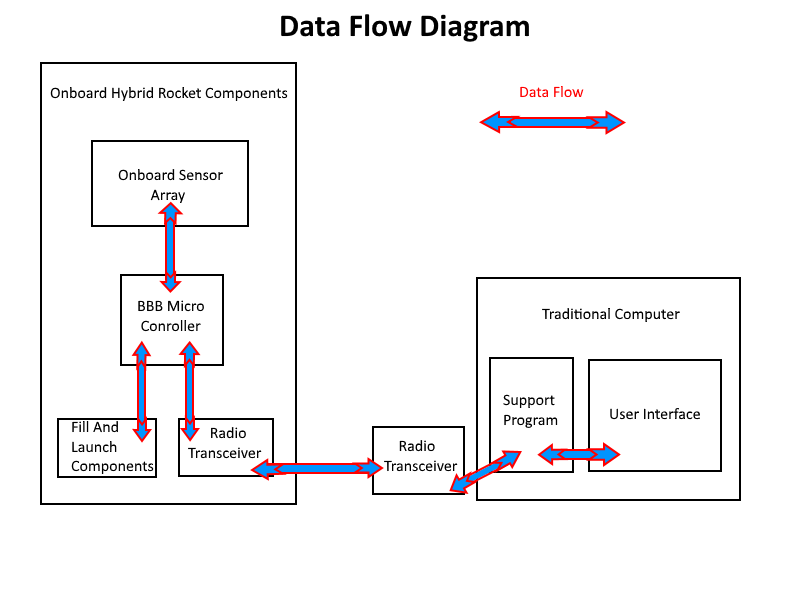
\includegraphics[scale=.85]{RocketBlockDiagram}
\end{figure}
\FloatBarrier

\subsection{Components} 

{\bf Josh Asher}
\\ \\
This section is intended to explain the electrical components of the rocket we will be receiving and/or sending data too. Most of the data collection will be coded by our ECE counter parts and passed to us to send to the ground unit. They have designed the electrical subsystem and written the drivers for the sensors. We will in turn make sure to receive this data and send their sub system commands from the ground. \par
Based on current design plans the rocket will have an accelerometer, barometric/temperature sensor, and a servo to control filling, arming, and launching of the rocket. The sensors will be polled by the ECE sub system and the data will be passed to us. The system is still in design fluctuation, but we for sure will be reciving altitude, pressure, temperature, and acceleration data.\par

\subsection{Data Format}
There are two buffers in this program. One to hold the sensor data and one to hold commands received. They are both globally available to the entire program.
\subsubsection{Sensor Data Buffer}
The sensor data buffers will be Python Queues; one for each data item. As data is received from the ECE sub system each data item will be placed in its respective queue. When the data is ready to send we remove the items from the Queue and place them into string to send. The size of this string will be limited by what the XBee radio transceivers will be able to transfer. This size has not completely been determined. Regardless when it comes time to transmit data we will empty the queues as needed to create as large of a data transmission as possible.

\begin{description}
	\item[Data Buffers] Queues that hold sensor information before processing.
	\item[Queue Names]  -
		\begin{description}
			\item[altitude] The altitude above ground level reading from the altitude sensor.
			\item[temp] The temperature reading from the temperature sensor.
			\item[a\_x] Accelerometer data from x axis.
			\item[a\_y] Accelerometer data from y axis.
			\item[a\_z] Accelerometer data from z axis.
			\item[g\_x] Gyroscope data from the x axis.
			\item[g\_y] Gyroscope data from the y axis.
			\item[g\_z] Gyroscope data from the z axis.
			\item[m\_x] Magnetometer data from the x axis.
			\item[m\_y] Magnetometer data from the x axis.
			\item[m\_z] Magnetometer data from the x axis.
			\item[tank\_pres] The pressure of the oxidizer tank. **This is a stretch goal at the moment.
			\item[chamber\_pres] The pressure of the combustion chamber. **This is a stretch goal at the moment.
		\end{description}
\end{description}
\subsubsection{Data Message Format}
The data that will be sent will be in a format agreed upon by the ECE and CS teams involved in this project. For the moment we have decided that commands will be sen in plain English and if there are more than one in a message they will be separated by commas. For example "Fill,Ignite" would be a legal command message. Data messages will be in a similar format. Only they will first be appended by the name of data and an equals sign. For example "a\_y=100,a\_x=235,a\_z1034,pressure=50" would be a legal data message.

\subsubsection{Command Buffer}
The command buffer will be used to store commands received from the ground computer software component to be accessed by the ECE subsystem for processing. A python queue will be used to provide first in first out behavior. When a command is detected it is added to this queue and as it is processed it is removed from the queue. The queue will be manipulated in the processing loop of the main thread.\par
 
\subsection{Methods and Threads}
This component will be designed in using multi threaded approach with helper functions. Each thread will be responsible for a certain aspect of the system. They will communicate through the two buffers detailed above. This will require mutex locks be put on the buffers prior to any action taken from the independent threads. The following is a list of the threads and helper functions with their descriptions and interactions. \par
\subsubsection{Sensor Polling Thread} 
{\bf Purpose:} \\
This thread is used to pull data from the sensors subsystem. The data is then placed into the sensor data buffer to be packed up and sent tot he radio transceiver. \par
{\bf Definition:} \\ 
sensor\_thread() \par
{\bf Inputs:} \\  Sensor data from the varies sensors from the ECE sub system. This input is read from a socket connected to the ECE sub system. Data comes in in the format mentioned above. \par
{\bf Outputs:} \\ Sensor data to the sensor data queues. \par
{\bf Process/Algorithm:} \\
This thread runs a continuous loop that waits to receive message from the ECE sub system socket. It then parses the message and places each sensor value in its respective queue. When the thread has collected data from all sensors it will place a mutex lock on the sensor data buffer and write the new data to the buffer. \par
\subsubsection{Command Processing Thread}
{\bf Purpose:} \\
The command processing thread will monitor for new commands from the radio transceiver. If commands are received it will process them and place them into the message format detailed above and send them to the ECE subsystem socket. The commands are stored in the command queue on arrival by the radio transceiver thread. The ECE subsystem from this point will act on the command. \par

{\bf Definition:} \\ 
command\_thread() \par
{\bf Inputs:} \\  Data from the command queue. \par
{\bf Outputs:} \\  Message to send to ECE subsystem socket and messages to rf\_send() \par
{\bf Calls:} \\ 
rf\_send(message)  \par
{\bf Process/Algorithm:} \\
The command processing thread will monitor the command queue for new commands. If the command queue length is not zero there is a new command in the buffer.The buffer will be checked  every 250 milliseconds for a new command. Commands will be processed through a set of conditional statements. Commands must be performed in a specific sequence detailed below next to the command explanation. Boolean flags will be used to determine if a command has been previously processed.  Once a command has processed it will be passed to the ECE subsystem through a socket for that subsystem to process and act on. This will result in physical responses by electrical components. \par
 After each command is successfully processed an acknowledgment will be sent to rf\_send(message) to inform the ground software a command was successfully processed. If a command does not pass a conditional, a message will be sent to radio transceiver by calling rf\_send(message) with the appropriate error message. The command will then be dropped and no action will be taken. Once the command sequence has been fulfilled the rocket is put into the launch state. This is dictated by a global boolean variable. Each command below is explained in regardless to what the ECE subsystem is supposed to accomplish when commands are sent to it.\par
{\bf Commands:} \\
\begin{description}
	\item[fill] This will adjust a servo to fill the oxidizer tank before launch. Sequence number 1.
	\item[arm] This will adjust a servo prepare the rocket for ignition. Sequence number 2.
	\item[ignition] This will send a signal to igniter to ignite the rocket fuel. Sequence number 3.
	\item[launch] This will adjust a servo to release the rocket from its base. Sequence number 4.
	\item[disarm] This will adjust a servo to reverse the arming process. Can be used at any time.
	\item[abort] This will adjust all servos to their initial state. Can be used at any time.
\end{description}
\subsubsection{Radio Transceiver Thread}
{\bf Purpose:} \\
The radio transceiver thread is responsible for monitoring the radio transceiver for incoming data from the software running on the traditional computer. It also monitors for data in the data queues and will form a message when enough is present and send it to the ground unit. \par
{\bf Definition:} \\ 
comm\_thread() \par
{\bf Inputs:} \\  Data from the radio transceiver and data from ECE subsystem. \par
{\bf Outputs:} \\ Data to the command buffer and data to the radio transceiver. \par
{\bf Calls:} \\ rf\_send(message) \par
{\bf Process/Algorithm:} \\
When the radio transceiver thread initializes it creates an XBee object with a call back function. This callback function is asynchronous and will be ran anytime a message is received by the XBee. This is all defined in xbee\_thread.py as a class that extends the python threading class. This object is instanciated in the initial main process. At this point the rocket is in a the pre-launch state which is dictated by a boolean flag. While the rocket is in the pre-launch stage this thread will only poll the radio transceiver object for new messages. When a command is received it is placed into the command buffer by first putting a mutex lock on the buffer and pushing the new command onto the queue. The thread will repeat this process until it detects that the pre-launch stage has passed.  \par
After the system has enter the launch stage this thread will change its behavior. Instead of monitoring for commands it will monitor the sensor data queues for new data every 500 milliseconds. It will place any data it finds in the data queues into a string in the format mentioned above then send the buffer into the radio transceiver by calling rf\_send(message) with the values from the dictionary as parameters. It repeats this process indefinitely. \par

\subsubsection{Main Thread}
{\bf Purpose:} \\
The main thread in the entry point into the software. It runs all initialization functions and starts all threads. \par
{\bf Definition:} \\ 
main() \par
{\bf Inputs:} \\  None \par
{\bf Outputs:} \\ None \par
{\bf Calls:} \\ init(), comm\_thread(), sensor\_thread(), command\_thread \par
{\bf Process/Algorithm:} \\
The main function calls the initialization function then creates the radio transceiver thread, the command processing thread, and the sensor thread. It will shut down all threads on program exit. \par
\subsubsection{Initialization Function}
{\bf Purpose:} \\
Initialize any threads, queues(buffers), or global variables. \par
{\bf Definition:} \\ 
init() \par
{\bf Inputs:} \\  None \par
{\bf Outputs:} \\ None \par
{\bf Process/Algorithm:} \\
Initializes all global variables to default values, creates the command and data queues, and initializes and start all threads. \par

\subsubsection{Radio Transceiver Send Function}
{\bf Purpose:} \\
Writes a message to send to the radio transceiver. \par
{\bf Definition:} \\ 
send\_rf(message) \par
{\bf Inputs:} \\  Message to send. \par
{\bf Outputs:} \\ Message to radio transceiver. \par
{\bf Process/Algorithm:} \\
Upon being called, in turn calls the write function of the radio transceiver object with the message provided in the message parameter. 
\subsection{Rationale}
Our projects major functions are to get data from a rocket to a traditional computer and represent it visually. As far as the software running on the beagle bone black its main function is to process commands and transmit sensor data. The approach we have taken will allow for fast easy maneuvering of data by using a multi threaded process that will store the data directly in memory. The threads will allow for simultaneous operation of these features. The approach we chose is procedural in many ways, but much of our threading code is oriented around classes. Our program will not be large compared to modern programs, but needs to perform specific tasks.

\subsection{Language}
We have chosen to use python because of its simplicity and strong API for USB reading and graphic rendering. It also is a stronger cross platform language then other options we explored. Another determining factor in this choice was last years success with this language. We have tested many of the aspects in python now and our ECE counter parts have also chosen this language. We have noticed that many of the components we have chosen come with python libraries ready to use. This allows us to easily communicate and between teams and help each other out. Python so far has proven to be very useful in solving the problem we have been presented with.

\section{System Architecture on a Traditional Computer }
The SDD module design of the software running on a traditional computer detailed here after will explain the approach, methods, and properties of this component of the system. Software running on the traditional computer will communicate to the software detailed above running on-board the rocket. This component of the system will be responsible for monitoring radio transmissions, sending commands, logging, replaying logged data, and the user interface back end. \par

\subsection{Overview}
In the following sections we describe the components of this software, excluding the user interface which is described in depth in the next section. We go over the graphical back end toolkits that will be used to draw the user interface, the data format of queues( buffers) and logs, worker threads, button listener functions, data conversion functions, and data visualization functions (drawing functions). \par

\subsection{GUI and Graphing Toolkits}
We will be using the Python TKinter library which provides a basis for windows, buttons, canvas, and other varies components we will need to create our graphical interface. This library includes event listeners to easily detect button presses and canvas to easily draw gauges and graphs. All sub components like buttons are called widgets in TKinter. \par
On top of Tkinter we will be using Matplotlib which is a graphical plotting library. Matplotlib provides functions to be easily able to graph data and scale those graphs. Graphs will be drawn on TKinter canvas widgets.\par

\subsection{Data Format}
\subsubsection{Sensor Data Buffer}
The sensor data buffer will be individual queues each relating to a sensor component on board the rocket.
\begin{description}
	\item[Sensor Data Queues]
	\item[Queue Names]  -
		\begin{description}
			\item[altitude] The altitude above ground level reading from the altitude sensor.
			\item[temp] The temperature reading from the temperature sensor.
			\item[chamber\_pres] The pressure of inside the chamber of the rocket body.
			\item[accell] Accelerometer data from x axis.
			\item[velocity] Derived velocity data from acceleration data.
			\item[tank\_pres] The pressure of the oxidizer tank.**This is a stretch goal
			\item[tank\_temp] The temperature of the oxidizer tank.**This is a stretch goal
			
		\end{description}
\end{description}
\subsubsection{Log Buffers}
Log buffers will hold previously received data for a particular queue from the sensor data buffer. Each queue (listed in the last section) will have its own buffer. As data is processed it will be placed into its log buffer. The log buffers will each hold up to 1024 of the last entries. This is to allow time graphs to be plotted. These buffers are regular arrays, one for each data queue.
\begin{description}
	\item[Buffers]  -
		\begin{description}
			\item[altitude] The altitude above ground level reading from the altitude sensor.
			\item[temp] The temperature reading from the temperature sensor.
			\item[chamber\_pres] The pressure of inside the chamber of the rocket body.
			\item[accell] Accelerometer data from x axis.
			\item[velocity] Derived velocity data from acceleration data.
			\item[tank\_pres] The pressure of the oxidizer tank.**This is a stretch goal
			\item[tank\_temp] The temperature of the oxidizer tank.**This is a stretch goal
		\end{description}
\end{description}

\subsubsection{Command Response Message Format}
Command response message will be sent as a string with the command that is being responded too followed by a colon followed then by the response message from the on-board system. All commands have not been finalized by the rocket team, but will follow this format.  For example: \par
{\bf Launch: Sequence has not been followed. Rocket is not ready to launch. } \par

\subsubsection{Data Log Format}
When data is logged each entry will be placed in separate text files named after the data item appended to the time it was created. Each entry will be separated by commas. The line will consist of a time stamp and then a list of key value pairs from the data buffer. Key value you pairs will have an equal sign between them. Data logs can then be ran back through to system by loading each individual entries. There will be an a menu in the main menu that allows to you to load this previously recorded data into the user interface. \par

\subsubsection{Command Log Format}
When commands are logged each entry will be placed on a separate line of a text file. Each use of the program will generate a new file, the name of the file will be datalog appended with a time stamp. Entries will be formatted like the example below. \par
Here is an example complete command log entry.\par
{\bf  6-1-2016:12:05:20 Abort}\par

\subsubsection{Response Log Format}
When responses are logged each entry will be placed on a separate line of a text file  Each use of the program will generate a new file, the name of the file will be responselog appended with a time stamp.. The line will consist of a time stamp followed by the command that was responded to followed by a colon with the response to the command appended to the end. Here is an example complete response log entry.\par
{\bf  6-1-2016:12:05:20 Ignite:Sequence has not been followed. Rocket not ready to ignite.}\par

\subsection{Methods and Threads}
This component will be designed using multi threaded approach with helper functions. Each thread will be responsible for a certain aspect of the system. They will communicate through the two buffers detailed above. This will require mutex locks be put on the buffers prior to any action taken from the independent threads. The following is a list of the threads and helper functions with their descriptions and interactions.

\subsubsection{XBee Thread}
The main thread in the entry point into the software. It runs all initialization functions and starts all threads. \par
{\bf Definition:} \\ 
xbee\_thread = xb\_rcv\_thread(1, "Xbee-Thread", 1, q=qu, port="COM4")  \par
{\bf Inputs:} \\  None \par
{\bf Outputs:} \\ None \par
{\bf Calls:} \\ Internal member functions listed in the class description below. \par
{\bf Process/Algorithm:} \\
This thread is an extended class of the threading class. Its purpose is to represent point of XBee communication. It sets up the radio transceiver and monitors the transceiver with a call back function. It also establishes a send function for the program to use to send data through the radio transceiver.  \par

\subsubsection{XBee Thread Class}
This class is used to establish an XBee object that is linked to the radio transceiver and provide listening/sending capabilities. \par

{\bf Member Methods:} \par

 \_\_init\_\_(self, threadID, name, counter, q, port) - \\ \\
This method initiates the class with the information in the parameters. Self refers the the instantiated class object, threadID is the id of he thread, name is the programmer provided name of the thread, counter is the number of the thread in the system, q is the queue place the received message on, and port is the USB port to open the communication on. \par

run(self) - \\ \\
This method is called when the thread starts and in turn starts the listening thread. \par

init(self) - \\ \\
This method initializes the serial port and returns its reference. \par

end(self) - \\ \\
This method is called when the thread needs to close in order to close the XBee communication and communications port. \par

listen(self) - \\ \\
This method is called when the thread starts and is responsible for keeping the thread alive. There is a call back function defined to listen for radio transmissions, but this function runs an endless while loop that keeps the thread alive until a call is made to close the thread. \par

processMessage(self, data) - \\ \\
This method is the callback function attached to the XBee API object. It is called when data is available on the XBee. This data is pushed onto the message queue.


\subsubsection{Main Thread}
{\bf Layne Nolli } 
\\ \\
The main thread in the entry point into the software. It runs all initialization functions and starts all threads. \par
{\bf Definition:} \\ 
main() \par
{\bf Inputs:} \\  None \par
{\bf Outputs:} \\ None \par
{\bf Calls:} \\ init(), data\_thread, redraw\_thread, xbee\_thread \par
{\bf Process/Algorithm:} \\
The main function calls the initialization function then creates the data thread and the redraw thread. It will shut down all threads on program exit. \par


\subsubsection{Data Thread}
The data thread is responsible form monitoring the message queue for new data. When new data is in the queue this thread it will parse the data  then pass it to the conversion method that will convert the data if needed. The Data Thread then stores the data in the appropriate data queue. Passing the command response messages to the command response function. \par
{\bf Definition:} \\ 
data\_thread() \par
{\bf Inputs:} \\  None \par
{\bf Outputs:} \\ New data to converter functions. \par
{\bf Calls:} \\ convTemp(data), convCHPressure(data), convAlititude(pressure, temp), convTankPressure(d), convAccell(data), convVelocity(data) \par
{\bf Process/Algorithm:} \\
The data thread continuously checks for data in the message queue that is filled by the xbee\_thread. When data is present in the queue this thread processes the data by parsing the message string. It locates the name of a data queue in the array and retrieves the value after the equals sign for that item. For example the string "temperature=68" would be parsed and 68 would be sent the to the convTemp() function. After conversion the data would be stored in the temperature queue. Which will be handled by the redraw thread from there on. If a command response message is received it is passed to the command response processing function.  \par

\subsubsection{Redraw Thread}
The redraw thread is responsible for monitoring for new converted data and passing the data to the appropriate redraw functions.\par
{\bf Definition:} \\
redraw\_thread() \par
{\bf Inputs:} \\  None \par
{\bf Outputs:} \\ None \par
{\bf Calls:} \\ drawTemp(data), drawCHPressure(data), drawAlititude(data), drawTankPressure(data), drawAccel(data), drawVelovity(data) \par
{\bf Process/Algorithm:} \\
The redraw thread will check a each data queue for new data. Upon detecting new data the redraw function will send each new data value to its appropriate draw function. After words removing the data from its queue. The data at this point has already been converted for the drawing functions so it may be passed directly to them. For example it will pass the temperature data from the data buffer to the drawTemp() function. This thread is only responsible for data delivery to the temperature, chamber pressure, altitude, tank pressure, acceleration, and velocity redraw functions. Each draw function is responsible for graphing the data to its specific canvas.\par

\subsubsection{Load Data Function}
{\bf Purpose:} \\
When ran opens log files and places their data into the data arrays for viewing on the user interface. \par
{\bf Definition:} \\ 
load\_data(logFile) \par
{\bf Inputs:} \\ Path to log defenition file that points to the right time stamp. \par
{\bf Outputs:} \\ Data to the data arrays, calls redraw functions. \par
{\bf Process/Algorithm:} \\
This function receives a path to a main log file. These files are named and contain the timestamp associated with the time the data was captured. It then selects each data file and loads them into the corresponding data array. Once the arrays are loaded it calls the redraw function to graph all the data. This is used for after launch analysis.\par

\subsubsection{Radio Transceiver Send Function}
{\bf Purpose:} \\
Writes a message to send to the radio transceiver. \par
{\bf Definition:} \\ 
send\_rf(message) \par
{\bf Inputs:} \\  Message to send. \par
{\bf Outputs:} \\ Message to radio transceiver. \par
{\bf Process/Algorithm:} \\
Upon being called in turns calls the write function of the radio transceiver object with the message provided in the message parameter. \par

\subsubsection{Initialization Function}
{\bf Purpose:} \\
Initializes global buffers, global objects, global variables, and the user interface. \par
{\bf Definition:} \\ 
init() \par
{\bf Inputs:} \\ None. \par
{\bf Outputs:} \\None. \par
{\bf Process/Algorithm:} \\
This function initializes all global buffers, objects and variables to their default values. It then creates the window object, all button widgets, all canvas widgets for graphs, and the graphing menu widget and buttons. Once all user interface items have been initialized it calls the main windows drawing method to display the initial interface. This function is called before any of the threads in this component are started. \par

\subsubsection{Process Command Response Function}
{\bf Purpose:} \\
Receives command response messages from the data thread and processes them. This function will inform the user of any failed or out of sequence commands and log the responses.  \par
{\bf Definition:} \\ 
command\_response(message) \par
{\bf Inputs:} \\  Command response to process. \par
{\bf Outputs:} \\ Logs responses to text file and message to screen. \par
{\bf Calls: drawMessage()}\par
{\bf Process/Algorithm:} \\
Upon receiving a command response message from the data thread this function opens the command response log and appends the message to the log with a newline. It then passes the message to the message draw function. \par

\subsubsection{Button Event Listeners}
Button listeners are provided by Tkinter as call back functions bound to the button the window. 

\paragraph{Command Button Listeners}
Each command button placed on the screen (shown in section 5) will have a function bound to it that will send the corresponding command string to the rf\_send() function. When a button is pressed that string is sent directly to the rf\_send function which in turn writes it to the radio transceiver. If a command fails the rocket will send a error response. It is not the responsibility of these functions to make sure the command is in the correct order. Below is an example command button callback function. \\ \\
{\bf sendFill() }
\\  \\
Each button will have its own functions like this. In this example the sendFill() function will call the rf\_send() function with the message "filll".

\subsubsection{Data Log Function}
{\bf Purpose:} \\
Logs the data it is passed to the data log text file.  \par
{\bf Definition:} \\ 
data\_log(data) \par
{\bf Inputs:} \\ Dictionary of data to log. \par
{\bf Outputs:} \\A line representing the data passed in to the data log text file. \par
{\bf Calls: drawMessage()}
{\bf Process/Algorithm:} \\
This function takes the data from data parameter and converts it to the data log format string. It then writes this string as a new line to the data log text file. \par

\subsubsection{Command Log Function}
{\bf Purpose:} \\
Logs the data it is passed to the command log text file.  \par
{\bf Definition:} \\ 
command\_log(data) \par
{\bf Inputs:} \\ Command to log. \par
{\bf Outputs:} \\A line representing the command passed in to the command log text file. \par
{\bf Calls: drawMessage()}
{\bf Process/Algorithm:} \\
This function takes the a command message from data parameter and converts it to the command log format string. It then writes this string as a new line to the command log text file. \par
\subsubsection{Converter Functions}
Each of the follow functions convert data they receive to the proper format for the drawing functions. They then store the data in the main data buffer for the drawing functions to access.  Each converter function is described in its specific details below. \par

\paragraph{Temperature Converter}
{\bf Purpose:} \\
Converts raw temperature sensor data to data suitable for the drawing functions.  \par
{\bf Definition:} \\ 
convTemp(data) \par
{\bf Inputs:} \\ Raw temperature data. \par
{\bf Outputs:} \\ Returns converted data. \par
{\bf Process/Algorithm:} \\
This function receives data from the data thread in its data parameter to convert to a temperature value suitable for graphing. It will convert the data by using a multiplier and offset provided on the data sheet of the temperature sensor.Temperature will be converted to Fahrenheit. \par

\paragraph{Chamber Pressure Converter}
{\bf Purpose:} \\
Converts raw pressure sensor data to data suitable for the drawing functions.  \par
{\bf Definition:} \\ 
convCHPressure(data) \par
{\bf Inputs:} \\ Raw chamber pressure data. \par
{\bf Outputs:} \\ Returns converted data. \par
{\bf Process/Algorithm:} \\
This function receives data from the data thread in its data parameter to convert to a pressure value suitable for graphing. It will convert the data by using a multiplier and offset provided on the data sheet of the pressure sensor used in the chamber of the rocket. Pressure will be converted to pounds per square inch. \par

\paragraph{Altitude Converter}
{\bf Purpose:} \\
Converts raw barometric pressure sensor readings to data suitable for the drawing functions.  \par
{\bf Definition:} \\ 
convAltitude(data) \par
{\bf Inputs:} \\ Raw barometric pressure data. \par
{\bf Outputs:} \\ Returns converted data. \par
{\bf Process/Algorithm:} \\
This function receives altitude data from the ECE subsystem. The altitude has already been processed by this subsystem and we need only use their provided multiplier and offset to correct it for our needs. \par

\paragraph{Tank Pressure Converter}
{\bf Purpose:} \\
Converts raw pressure sensor data to data suitable for the drawing functions.  \par
{\bf Definition:} \\ 
convTankPressure(data) \par
{\bf Inputs:} \\ Raw tank pressure data. \par
{\bf Outputs:} \\ Returns converted data. \par
{\bf Process/Algorithm:} \\
This function receives data from the data thread in its data parameter to convert to a pressure value suitable for graphing. It will convert the data by using a multiplier and offset provided on the data sheet of the pressure sensor used on the oxidizer tank of the rocket. Pressure will be converted to pounds per square inch. \par

\paragraph{Acceleration Converter}
{\bf Purpose:} \\
Converts raw accelerometer sensor data to data suitable for the drawing functions.  \par
{\bf Definition:} \\ 
convAccell(data) \par
{\bf Inputs:} \\ Raw acceleration data. \par
{\bf Outputs:} \\ Returns converted data. \par
{\bf Process/Algorithm:} \\
This function receives data from the data thread in its data parameter to convert to an acceleration value suitable for graphing. The parameter will be a raw acceleration reading from the sensor. It will convert this to the Meters per second squared with the formula provided by the sensor manufacturer. \par

\paragraph{Velocity Converter}
{\bf Purpose:} \\
Converts raw acceleration data to velocity data suitable for the drawing functions.  \par
{\bf Definition:} \\ 
convVelocity(data) \par
{\bf Inputs:} \\ Raw acceleration data. \par
{\bf Outputs:} \\ Returns converted data. \par
{\bf Process/Algorithm:} \\
This function receives data from the data thread in its data parameter to convert to a velocity value suitable for graphing. The parameter will be a raw acceleration reading from the sensor. It will convert this to the Meters per second by first converting it to meters per second squared (normal acceleration) with the formula provided by the sensor manufacturer. Then it will take the integral of the acceleration to obtain the velocity.\par

\subsubsection{Drawing Functions and Classes}\

{\bf Jason Klindtworth }
\\ \\
Each of the following drawing functions are called by the redraw thread when data becomes available to be displayed on the screen. They do not take data as input to be displayed, but instead read the data from the data queues or the larger data arrays. Except for the message drawing routing it takes a input message to be drawn in the message window. Each function is responsible for a different data item and will display it according to the format of that data. The following is a list of the drawing functions and their specific operation. Each of the routines below are part of canvas class associated with the widget and inherit all from one parent redraw function. The redraw function will be called on the canvas object that it associated with as mentioned above.

\subsubsection{Canvas Widget Class}
This class is used to provided a template for gauge drawing classes.

{\bf Member Methods:} \par

 \_\_init\_\_(self, mainwindow, x, y, w, h) - \\ \\
This method initializes object variables with the parameters provided by the calling function. Self is a reference to the object, mainwindow is a reference to the main TKinter window, x is the desired x position of the object on the user interface, y is the desired y position on the user interface, w is the width of the object, and h is the height. \par

putScreen(self) - \\ \\
This method places the widget on the user interface. \par

redraw(self) - \\
This method defines a template for other drawing routines that inherit from this class.

\subsubsection{Plot Widget Class}
This class is used to provided a template for drawing graphs. It is very similar to the canvas widget class, but it creates a Matplotlib object and attaches it to a canvas. Versus drawing something on a canvas directly.

{\bf Member Methods:} \par

 \_\_init\_\_(self, mainwindow, x, y, w, h) - \\ \\
This method initializes object variables with the parameters provided by the calling function. Self is a reference to the object, mainwindow is a reference to the main TKinter window, x is the desired x position of the object on the user interface, y is the desired y position on the user interface, w is the width of the object, and h is the height. \par

putScreen(self) - \\ \\
This method places the widget on the user interface. \par

redraw(self) - \\
This method defines a template for other drawing routines that inherit from this class.


\paragraph{Message Drawing Routine}
{\bf Purpose:} \\
Display command response message in the message window.  \par
{\bf Definition:} \\ 
drawMessage(message) \par
{\bf Inputs:} \\ Message string to draw.\par
{\bf Outputs:} \\Message to the message window. \par
{\bf Process/Algorithm:} \\
This function will take as its input parameter a command message and then draw the string in the message window of the user interface. \par

\paragraph{Temperature Drawing Routine}
{\bf Purpose:} \\
Draw the temperature data on the user interface.  \par
{\bf Definition:} \\ 
drawTemp() \par
{\bf Inputs:} \\None. \par
{\bf Outputs:} \\Temperature gauge on the user interface.\par
{\bf Process/Algorithm:} \\
This function will pull temperature data from the temperature queue and draw a gauge representing the data on the temperature canvas. \par

\paragraph{Chamber Pressure Drawing Routing}
{\bf Purpose:} \\
Draw chamber pressure on the user interface. \par
{\bf Definition:} \\ 
drawCHPressure() \par
{\bf Inputs:} \\None. \par
{\bf Outputs:} \\Chamber pressure gauge on the user interface.\par
{\bf Process/Algorithm:} \\
This function will pull chamber pressure data from the chamber pressure que and draw a gauge representing the data on the chamber pressure canvas. \par

\paragraph{Altitude Drawing Routine}
{\bf Purpose:} \\
Draw rocket altitude on the user interface. \par
{\bf Definition:} \\ 
drawAltitude() \par
{\bf Inputs:} \\None. \par
{\bf Outputs:} \\Altitude graph on the user interface.\par
{\bf Process/Algorithm:} \\
This function will pull altitude data from the altitude queue and draw a graph representing the data on the altitude canvas. \par

\paragraph{Tank Pressure Drawing Routine **Strech Goal}
{\bf Purpose:} \\
Draw oxidizer tank pressure on the user interface. \par
{\bf Definition:} \\ 
drawTankPressure() \par
{\bf Inputs:} \\None. \par
{\bf Outputs:} \\Oxidizer tank pressure gauge on the user interface.\par
{\bf Process/Algorithm:} \\
This function will pull tank pressure data from the tank pressure queue and draw a gauge representing the data on the tank pressure canvas. \par

\paragraph{Acceleration Drawing Routine}
{\bf Purpose:} \\
Draw acceleration graph on the user interface. \par
{\bf Definition:} \\ 
drawAccell() \par
{\bf Inputs:} \\None. \par
{\bf Outputs:} \\Acceleration graph on the user interface.\par
{\bf Process/Algorithm:} \\
This function will pull acceleration data from the acceleration queue and draw a graph representing the data on the acceleration canvas. \par

\paragraph{Velocity Drawing Routine}
{\bf Purpose:} \\
Draw velocity graph on the user interface. \par
{\bf Definition:} \\ 
drawVelocity() \par
{\bf Inputs:} \\None. \par
{\bf Outputs:} \\Velocity graph on the user interface.\par
{\bf Process/Algorithm:} \\
This function will pull velocity data from the velocity queue and draw a graph representing the data on the velocity canvas. \par

\paragraph{Draw Temperature Routine}
{\bf Purpose:} \\
Draws temperature vs time as graph on the user interface. \par
{\bf Definition:} \\ 
drawTempAsGraph() \par
{\bf Inputs:} \\None. \par
{\bf Outputs:} \\Temperature vs time graph on the user interface.\par
{\bf Process/Algorithm:} \\
This function will take multiple data points from the temperature log buffer and plot them vs time on the user interface in the time graph canvas.  \par

\paragraph{Draw Chamber Pressure Routine}
{\bf Purpose:} \\
Draws chamber pressure vs time as graph on the user interface. \par
{\bf Definition:} \\ 
drawCHPAsGraph() \par
{\bf Inputs:} \\None. \par
{\bf Outputs:} \\Chamber pressure vs time graph on the user interface.\par
{\bf Process/Algorithm:} \\
This function will take multiple data points from the chamber pressure log buffer and plot them vs time on the user interface in the time graph canvas.  \par

\paragraph{Draw Altitude Routine}
{\bf Purpose:} \\
Draws altitude vs time as graph on the user interface. \par
{\bf Definition:} \\ 
drawAltAsGraph() \par
{\bf Inputs:} \\None. \par
{\bf Outputs:} \\Altitude vs time graph on the user interface.\par
{\bf Process/Algorithm:} \\
This function will take multiple data points from the altitude log buffer and plot them vs time on the user interface in the time graph canvas.  \par

\paragraph{Draw Tank Pressure Routine}
{\bf Purpose:} \\
Draws tank pressure vs time as graph on the user interface. \par
{\bf Definition:} \\ 
drawTankPAsGraph()\par
{\bf Inputs:} \\None. \par
{\bf Outputs:} \\Tank pressure vs time graph on the user interface.\par
{\bf Process/Algorithm:} \\
This function will take multiple data points from the tank pressure log buffer and plot them vs time on the user interface in the time graph canvas.  \par

\subsection{Rationale}
This part of our system reads and sends data. A big part of this decision was the choice on Python. There are great graphics libraries available for Python that are tailored to our needs. Including the XBee Python API that we use to communicate with the radio transceiver. This library has proven a very effective way to use the XBees. The back end is a procedural based multi threaded system that provides simplicity and easy data access.

\subsection{Language}
We have chosen to use python because of its simplicity and strong API for USB reading and graphic rendering. It also is a stronger cross platform language then other options we explored. Another determining factor in this choice was last years success with this language and the ECE team shared the same choice for a language.

\section{User Interface Design}
The graphical user interface is the driving force behind this entire project. It may not seem as complicated as some modern interfaces, but its serves a very important purpose. The purpose is to visually represent data from a hybrid rocket and provide button to issue the rocket commands. It will also have the ability to load old data and graph it. These functions have been lacking in previous years rockets team and are the reason we were brought on board this project. Detailed in the following sections are these sections of the user interface. \par

\begin{itemize}
\item The Command Buttons
\item The Message Frame
\item The Gauges and  Graphs
\item The Load Menu
\end{itemize}

\subsection{Drawing of Complete Screen}
Here is a basic drawing of the entire screen. This drawing will be replaced with a screen shot once the program has reached a stage where the components are all visible.\par

\begin{figure}[!ht]
  \caption{Mock up of the graphical user interface}
  \centering
	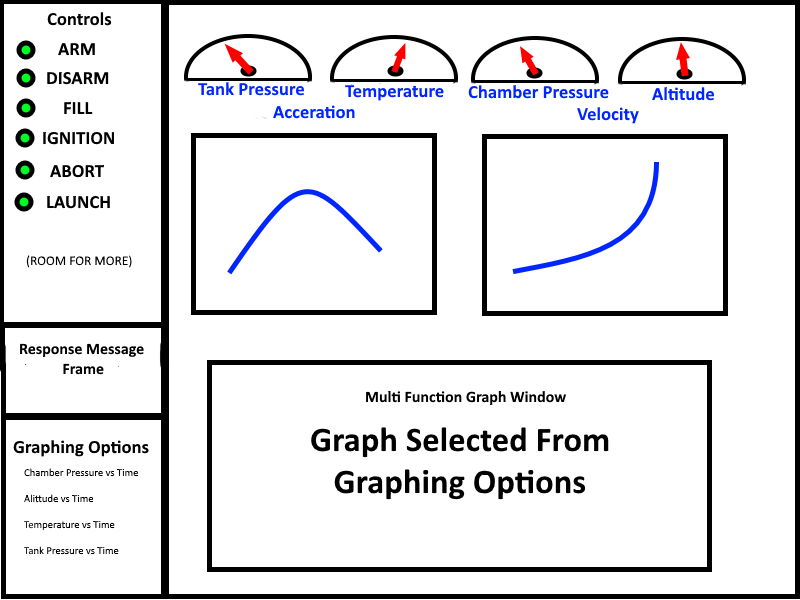
\includegraphics[scale=.85]{HyRoUIMockup}
\end{figure}

\subsection{The Command Buttons}
The command buttons are housed on the left side of the screen as depicted in the image above. These buttons will cause a command to be sent through the radio transceiver on the traditional computer to the radio transceiver on-board the rocket. The rocket will process the command and send a response back to be displayed in the message frame. The command buttons and their descriptions are as follows.\par

\begin{description}
\item[Fill] This will attempt to initiate the oxidizer fill process while the rocket is on the ground.
\item[Arm] This will adjust a servo prepare the rocket for ignition. Sequence number 2.
\item[Ignition] This will send a signal to igniter to ignite the rocket fuel. Sequence number 3.
\item[Launch] This will adjust a servo to release the rocket from its base. Sequence number 4.
\item[Disarm] This will adjust a servo to reverse the arming process. Can be used at any time.
\item[Abort] This will adjust all servos to their initial state. Can be used at any time.
\end{description}

\subsection{The Message Frame}
This is a small message box on the left hand side of the user interface directly under the command buttons. This box will display response message from the rocket. As message come in they will be appended to this message box. The box will be able to scroll if the messages exceeded the size of the frame.\par

\subsection{The Load Menu}
A small menu will be provided at the top left hand side of the screen. It will bring up a file explorer window and allow you to chose what old data to load. This will initiate the data loading routines and the redraw functions.

\subsection{The Gauges and Graphs}
Taking up most of the user interface on the right hand side are the gauges and graph canvases. Currently their will be 3 gauges that look like traditional gauges you would see on car dash board. They will be a semi circle with marks representing possible values of the data item. A arrow will be draw to represent the current value of the data. Below those gauges are 5 graphs representing all the different data items as graphs. Listed below are the gauges, graphs, and their units.

\subsubsection{Tank Pressure Gauge **Stretch goal}
{\bf Units} \\ Tick marks are measured in pounds per square inch from 0 to 2000.\par
{\bf Description} \\ This gauge represents the current pressure of the oxidizer tank. It will rise and fall along with the tank pressure. This value can also be graphed in the multifunction window.\par

\subsubsection{Temperature Gauge}
{\bf Units} \\ Tick marks are measured in degrees Fahrenheit from 32 to 7000.\par
{\bf Description} \\ This gauge represents the temperature wherever the temperature sensor is located. It will rise and fall along with the temperature surrounding the temperature sensor. This value can also be graphed in the multifunction window. \par

\subsubsection{Chamber Pressure Gauge}
{\bf Units} \\ Tick marks are measured in pounds per square inch from 0 to 2000.\par
{\bf Description} \\ This gauge represents the pressure of the combustion chamber of the rocket. It will rise and fall along with the chamber pressure of the rocket. This value can also be graphed in the multifunction window. \par

\subsubsection{Altitude Graph}
{\bf Units} \\ Time vs altitude graph. Altitude is displayed from 0 to 15000 feet.\par
{\bf Description} \\ This graph represents the altitude of the rocket. It will plot the altitude of the rocket vs time. \par

\subsubsection{Acceleration Graph}
{\bf Units} \\ The x axis of the graph will be measured in meters per second squared and the y axis will be time from launch in seconds.\par
{\bf Description} \\ This graph represents the acceleration of the rocket with respect to time. The graph will be able to slide if the amount of data points exceeds the size of the graph window. \par

\subsubsection{Velocity Graph}
{\bf Units} \\ The x axis of the graph will be measured in meters per second and the y axis will be time from launch in seconds.\par
{\bf Description} \\ This graph represents the velocity of the rocket with respect to time. The graph will be able to slide if the amount of data points exceeds the size of the graph window. \par

\subsubsection{Temperature Graph}
{\bf Units} \\ The x axis of the graph will be measured in Fahrenheit and the y axis will be time from launch in seconds.\par
{\bf Description} \\ This graph represents temperature over time of the avionics bay in the rocket. The graph will be able to slide if the amount of data points exceeds the size of the graph window. \par

\subsubsection{Pressure Graph}
{\bf Units} \\ The x axis of the graph will be measured pounds per square inch and the y axis will be time from launch in seconds.\par
{\bf Description} \\ This graph represents the pressure over time of the rocket. The graph will be able to slide if the amount of data points exceeds the size of the graph window. \par


\section{Summary}
The previous section have in detailed described our hybrid rockets software system. We have described how we will collect sensors data, send sensor data, receive and act on commands, and provide  a command and visualization interface for the rocket team members on the ground. We have detailed the data formats, log formats, radio transceiver routines, data conversion routines, drawing routines and the threads that will control all these components. These are all housed in a threaded procedural system for simplicity and speed. All these components combined will allow for remote filling, launching, and data visualization of a hybrid rocket. \par

\newpage

\section{Bibliography}
\begin{thebibliography}{9}

\bibitem{BBB}
 BeagleBone.org,\\
\emph{(Tues November 29 2016)},\\
  \emph{Beagle Bone Black product information and website},\\
URL  http://beagleboard.org/black \\

\bibitem{ExampleSDD}
Unimap.edu example SDD,\\
\emph{(Tues November 29 2016)}, \\
  \emph{Unimap software development examples}, \\
URL http://portal.unimap.edu.my/portal/page/portal30/Lecturer\%20Notes/KEJURUTERAAN\_KOMPUTER/Semester\%202\%20Sidang\%20Akademik\%2020112012/EKT420\%20Software\%20Engineering/Example\%20of\%20Software\%20Design\%20Document(SDD)/EDDISS.pdf \\

\bibitem{IEE1016}
IEE 1016 Software Design Specifications,\\
\emph{(Tues November 29 2016)}, \\
  \emph{IEE 1016 Document availble on campus}, \\

\bibitem{TKinter}
Python.org wiki,\\
\emph{(Tues November 29 2016)}, \\
  \emph{Tkinter python wiki on python.org}, \\
URL https://wiki.python.org/moin/TkInter\\

\bibitem{Matplotlib}
Matplotlib.org,\\
\emph{(Tues November 29 2016)}, \\
  \emph{Matplotlib.org website documentation}, \\
URL http://matplotlib.org/

\end{thebibliography}

\newpage
\textbf{Students:}

\vspace{5mm}
 

\noindent \namesigdate{Jason Klindtworth} \hfill \namesigdate[6cm]{Josh Asher}
\vspace{5mm}

\noindent \namesigdate{Layne Nolli}
 \vspace{5mm}

\textbf{Client:}

\vspace{5mm}
 

\noindent \namesigdate{Nancy Squires}


\end{document}
